\documentclass[12pt,a4paper]{article}
\usepackage{ctex}
\usepackage{amsmath,amscd,amsbsy,amssymb,latexsym,url,bm,amsthm}
\usepackage{epsfig,graphicx,subfigure}
\usepackage{enumitem,balance}
\usepackage{wrapfig}
\usepackage{mathrsfs,euscript}
\usepackage[usenames]{xcolor}
\usepackage{hyperref}
\usepackage[vlined,ruled,linesnumbered]{algorithm2e}
\hypersetup{colorlinks=true,linkcolor=black}

\newtheorem{theorem}{Theorem}
\newtheorem{lemma}[theorem]{Lemma}
\newtheorem{proposition}[theorem]{Proposition}
\newtheorem{corollary}[theorem]{Corollary}
\newtheorem{exercise}{Exercise}
\newtheorem*{solution}{Solution}
\newtheorem{definition}{Definition}
\theoremstyle{definition}

\renewcommand{\thefootnote}{\fnsymbol{footnote}}

\newcommand{\postscript}[2]
 {\setlength{\epsfxsize}{#2\hsize}
  \centerline{\epsfbox{#1}}}

\renewcommand{\baselinestretch}{1.0}

\setlength{\oddsidemargin}{-0.365in}
\setlength{\evensidemargin}{-0.365in}
\setlength{\topmargin}{-0.3in}
\setlength{\headheight}{0in}
\setlength{\headsep}{0in}
\setlength{\textheight}{10.1in}
\setlength{\textwidth}{7in}
\makeatletter \renewenvironment{proof}[1][Proof] {\par\pushQED{\qed}\normalfont\topsep6\p@\@plus6\p@\relax\trivlist\item[\hskip\labelsep\bfseries#1\@addpunct{.}]\ignorespaces}{\popQED\endtrivlist\@endpefalse} \makeatother
\makeatletter
\renewenvironment{solution}[1][Solution] {\par\pushQED{\qed}\normalfont\topsep6\p@\@plus6\p@\relax\trivlist\item[\hskip\labelsep\bfseries#1\@addpunct{.}]\ignorespaces}{\popQED\endtrivlist\@endpefalse} \makeatother

\begin{document}
\noindent

%========================================================================
\noindent\framebox[\linewidth]{\shortstack[c]{
\Large{\textbf{Lab02-Divide and Conquer}}\vspace{1mm}\\
CS214-Algorithm and Complexity, Xiaofeng Gao, Spring 2020.}}
\begin{center}
\footnotesize{\color{red}$*$ If there is any problem, please contact TA Yiming Liu.}

% Please write down your name, student id and email.
\footnotesize{\color{blue}$*$ Name:Hongjie Fang  \quad Student ID:518030910150 \quad Email: galaxies@sjtu.edu.cn}
\end{center}

\begin{enumerate}
    \item
    \textbf{Quicksort} is based on the Divide-and-Conquer method. Here is the two-step divide-and-conquer process for sorting a typical subarray $A[p \ldots r]$:
    \begin{enumerate}

    	\item
    	\textbf{Divide:} Partition the array $A[p \ldots r]$ into two subarrays $A[p \ldots q-1]$ and $A[q+1 \ldots r]$ such that each element of $A[p \ldots q-1]$ is less than or equal to $A[q]$, which is, in turn, less than or equal to each element of $A[q+1 \ldots r]$. Compute the index $q$ as part of this partitioning procedure.
    	
    	\item
    	\textbf{Conquer:} Sort $A[p \ldots q-1]$ and $A[q+1 \ldots r]$ respectively by recursive calls to Quicksort.
    	
    \end{enumerate}
    Write down the recurrence function $T(n)$ of QuickSort and compute its time complexity.

    {\color{purple}Hint: At this time $T(n)$ is split into two subarrays with different sizes (usually), and you need to describe its recurrence relation by the sum of two subfunctions plus additional operations.}

    \begin{solution}
    Assume the recurrence function $T(n)$ stands for total operation times of Quicksort, where $n$ denotes the current length of the array (i.e., $n = r - p + 1$). Suppose we choose the pivot $A[q]$ in a time complexity of $O(1)$, and finish the partition in a time complexity of $O(n)$. We consider the best case, the worst case and the average case of the Quicksort.
    \begin{itemize}
    \item \textbf{The best case:} The best case happens when every time we take a partition, two parts ($A[p \ldots q-1]$ and $A[q+1 \ldots r]$) have almost the same size, which indicates that $q$ equals to $\lfloor \frac{p + r}{2} \rfloor$ in every partitioning procedure. Then suppose the original length of the array is $n$ before partition, and after partition we will get two sub-arrays of length $\left\lfloor \frac{n}{2} \right\rfloor$ each. Thus, we can derive the following equation (Equation \eqref{eq1:1}).
        \begin{equation}
          T(n) = \left\{
          \begin{aligned}
          & 0 & \quad \quad \mathrm{if\ } n = 1 \\
          & 2 T\left(\left\lfloor \frac{n}{2} \right\rfloor \right) + O(n) & \quad \quad \mathrm{if\ } n > 1
          \end{aligned}
          \right.
          \label{eq1:1}
        \end{equation}
        We can derive that $T(n) = O(n\log{n})$ using Master Theorem. So the best case of Quicksort has a time complexity of $O(n\log{n})$.
    \item \textbf{The worst case:} The worst case happens when every time we take a partition, one of the two parts ($A[p \ldots q-1]$ and $A[q+1 \ldots r]$) is empty, which indicates that $q$ equals to either $p$ or $r$. Then suppose the original length of the array is $n$ before partition, and after partition we will get an empty sub-array and a sub-array of length $(n - 1)$. Thus, we can derive the following equation (Equation \eqref{eq1:2}).
        \begin{equation}
          T(n) = \left\{
          \begin{aligned}
          & 0 & \quad \quad \mathrm{if\ } n = 1 \\
          & T(n - 1) + O(n) & \quad \quad \mathrm{if\ } n > 1
          \end{aligned}
          \right.
          \label{eq1:2}
        \end{equation}
        We can derive that $T(n) = O(n^2)$ using simple mathematical knowledge. So the worst case of Quicksort has a time complexity of $O(n^2)$.
    \item \textbf{The average case:} When considering the average case of the Quicksort, we assume that every possible partition happens equally likely. Suppose one of the two parts ($A[p \ldots q-1]$ and $A[q+1 \ldots r]$) has a length $i\ (0 \leq i < n)$, then the other part has a length $(n - i - 1)$. There are total $n$ possibilities and each has a probability of $\frac{1}{n}$. Thus, we can derive the following equation (Equation \eqref{eq1:3}).
        \begin{equation}
          T(n) = \left\{
          \begin{aligned}
          & 0 & \quad \quad \mathrm{if\ } n = 1 \\
          & O(n) + \sum_{i=0}^{n-1}\frac{1}{n} \cdot (T(i) + T(n - i - 1)) & \quad \quad \mathrm{if\ } n > 1
          \end{aligned}
          \right.
          \label{eq1:3}
        \end{equation}
        We can simplify the Equation \eqref{eq1:3} and make some mathematical derivation as follows.
        \begin{displaymath}
          \begin{aligned}
          \frac{n}{n-1} \cdot T(n) - T(n-1)  &= \frac{2}{n-1} \left(\sum_{i=0}^{n-1} T(i) - \sum_{i=0}^{n-2} T(i)\right) + O(1) \\
                                             &= \frac{2}{n-1} \cdot T(n-1) + O(1) \quad \quad (n > 1)\\
          \Longrightarrow \quad \quad T(n) &= \frac{n+1}{n} \cdot T(n-1) + O(1) \quad \quad (n > 1)
          \end{aligned}
        \end{displaymath}
        Solve the recurrence equation above, we can get that $T(n) = H(n) \cdot O(n)$, where $H(n)$ is the sum of the first $n$ terms of the harmonic series. Therefore, we can derive that $T(n) = O(n\log{n})$ using the Euler's conclusion that $H(n) \sim \log{n}$. So the average case of Quicksort has a time complexity of $O(n\log{n})$.
    \end{itemize}
    \end{solution}

    \clearpage
    \item
    \textbf{MergeCount}. Given an integer array $A[1 \ldots n]$ and two integer thresholds $t_l \le t_u$, Lucien designed an algorithm using divide-and-conquer method (As shown in Alg.~\ref{Alg-MergeCount}) to count the number of ranges $(i,j)$ ($1 \leq i \leq j \leq n$) satisfying
    \begin{equation}\label{Eqn-MergeCount}
    t_l \leq \sum_{k=i}^{j}{A[k]} \leq t_u.
    \end{equation}

    Before computation, he firstly constructed $S[0 \ldots n+1]$, where $S[i]$ denotes the sum of the first $i$ elements of $A[1 \ldots n]$. Initially, set $S[0]=S[n+1]=0$, $low=0$, $high=n+1$.

    \begin{minipage}[t]{0.90\textwidth}
	\begin{algorithm}[H]
		%\algsetup{footnotesize}
		%\scriptsize
		\KwIn{$S[0,\cdots,n+1]$, $t_l$, $t_u$, $low$, $high$.}
		\KwOut{$count$ = number of ranges satisfying Eqn.~\eqref{Eqn-MergeCount}.}
		\BlankLine
		\caption{MergeCount($S$, $t_l$, $t_u$, $low$, $high$)}
		\label{Alg-MergeCount}
		
		$count \leftarrow 0$; $mid\leftarrow \lfloor \frac{low+high}{2} \rfloor$\;
		
		\lIf{$mid=low$}{
			\Return{$0$}
		}
		
		$count\leftarrow MergeCount(S, t_l, t_u, low, mid)+ MergeCount(S, t_l, t_u, mid, high)$\;
		
		\For{$i = low$ \textbf{to} $mid-1$}{
			$m \leftarrow \left \{ \begin{array}{ll}
            \min\{m \mid S[m]-S[i] \ge t_l, m \in [mid, high-1]\}, & \text{if exists}\\
            high, & \text{if not exist}
            \end{array}\right.$\;
			
			$n \leftarrow \left \{ \begin{array}{ll}
            \min\{n \mid S[n]-S[i] > t_u, n \in [mid, high-1]\}, & \text{if exists}\\
            high, & \text{if not exist}
            \end{array}\right.$
			\tcp*[r]{\color{blue}BinarySearch is used to find $m$, $n$}
			$count \leftarrow count+n-m$\;
		}
		$Merge(S,low,mid-1,high-1)$  \tcp*[r]{\color{blue}Merge is used for two sorted arrays}
		
		\Return{$count$}\;
		
	\end{algorithm}
    \end{minipage}

    {\color{purple}\textbf{Example:} Given $A = [1,-1,2]$, $lower = 1$, $upper = 2$, return 4. The resulting four ranges should be $(1,1)$, $(1,3)$, $(2,3)$, and $(3,3)$.}

    Is Lucien's algorithm correct? Explain his idea and make correction if needed. Besides, compute the running time of Alg.~\ref{Alg-MergeCount} (or the corrected version) by recurrence relation. {\color{blue}(Note: we can't implement Master's Theorem in this case. Refer Reference06 for more details.)}

    \begin{solution}
        Lucien's algorithm is \textbf{correct}. Here is Lucien's idea.
        \begin{itemize}
        \item Notice that every pair $(S[i], S[j])\ (0 \leq i < j \leq n)$ represents a range $(i, j]$, and the sum of elements in it is $(S[j] - S[i])$ (i.e., $\sum_{k=i+1}^j A[k] = S[j] - S[i]$). And also every range can be represent as a pair $(S[i], S[j])\ (0 \leq i < j \leq n)$. Hence, we are going to count the number of pairs $(S[i], S[j])\ (0 \leq i < j \leq n)$ satisfying $t_l \leq S[j] - S[i] \leq t_u$.
        \item Assume that current process is $MergeCount(S, t_l, t_u, low, high)$, in which we want to count the number of pairs with indexes in $[low, high)$ that satisfy the conditions above, then let $mid$ be $\left\lfloor \frac{low + high}{2} \right\rfloor$. Divide the current interval into two small sub-intervals, which are $[low, mid)$ and $[mid, high)$.
        \item Assume that pairs we concern about is $(S[i_1], S[j_1]), (S[i_2], S[j_2]), ..., (S[i_m], S[j_m])$, and we want to check whether these pairs satisfy the condition. Obviously, the indexes of these ranges must be in the current interval, that is, $i_k, j_k \in [low, high) \ (1 \leq k \leq m)$. Divide these pairs into three parts:
        \begin{itemize}
        \item \textbf{Situation I:} Pairs with both indexes in the left sub-interval, that is, all the pairs $(S[i_k], S[j_k])\ (1 \leq k \leq m)$ satisfying $low \leq i_k < j_k < mid$;
        \item \textbf{Situation II:} Pairs with both indexes in the right sub-interval, that is, all the pairs $(S[i_k], S[j_k])\ (1 \leq k \leq m)$ satisfying $mid \leq i_k < j_k < high$;
        \item \textbf{Situation III:} Pairs with indexes crossing two sub-intervals, that is, all the pairs $(S[i_k], S[j_k])\ (1 \leq k \leq m)$ satisfying $low \leq i_k < mid \leq j_k < high$.
        \end{itemize}
            These three situations contain all the pairs we concern about, and every two situations have a empty intersection set of pairs. Thus, this divide method is correct.
        \item Situation I and Situation II are easy to solve, since we can count the number of pairs by calling $MergeCount(S, t_l, t_u, low, mid)$ and $MergeCount(S, t_l, t_u, mid, high)$ recursively.
        \item Situation III is a little bit difficult, so we use the following method to count the number of pairs.
        \begin{itemize}
        \item We enumerate $i$ from $low$ to $(mid - 1)$ to count the number of pairs with the first element being $S[i]$ (i.e., pairs in this pattern $(S[i], \cdot)$).
        \item Given the first index $i$, we want to count the number of indexes $j\ (mid \leq j < high)$ satisfying $t_l + S[i] \leq S[j] \leq t_u + S[i]$.
        \item Now assume $S[mid \ldots high]$ is already sorted, then the problem can be solved by binary search (search the beginning index and the ending index that satisfy the condition, then all the indexes between them are valid) with a time complexity of $O(\log{(high - mid)})$ each time.
        \end{itemize}
        \item Now we come back to the assumptions we make above. We need the array $S$ be sorted. Notice that the framework of the algorithm is similar to MergeSort, so we call the function merge in MergeSort to merge two already-sorted part $S[low \ldots mid]$ and $S[mid \ldots high]$ together. Therefore, the assumption in situation III is satisfied.
        \item Combining the number of pairs in Situation I, II, III together, we can get the number of pairs with indexes in $[low, high)$ that satisfy the conditions.
        \item \textbf{Explanation of correctness:} The main point of the correctness proof is that whether the sorting process will affect the answer, and the answer is no. Every time we count the pairs in Situation III, we have fix their left index in left sub-interval and right index in right sub-interval, so left index is bound to be less than the right index. When counting pairs, we do not care about the original places of indexes in the sub-intervals. Thus, the sorting processes of the left sub-interval and the right sub-interval have no effect on the answer. Thus the correctness of sorting process in the algorithm is proved.
        \end{itemize}
        \textbf{The Time Complexity:} Now we compute the time complexity of the algorithm. Assume the recurrence function is $T(n)$ with $n = high - low$, then we can derive the equation as follows (Equation \eqref{eq2:1}).
        \begin{equation}
        T(n) = \left\{
        \begin{aligned}
        & 0 & \quad \quad \mathrm{if\ } n = 1 \\
        & 2T\left(\left\lceil \frac{n}{2} \right\rceil\right) + O(n \log{n}) &  \quad \quad \mathrm{if\ } n > 1
        \end{aligned}
        \right.
        \label{eq2:1}
        \end{equation}
        Then we can unfold the recurrence equation as follows (Equation \eqref{eq2:2}).
        \begin{equation}
        \begin{aligned}
        T(n) &= 2T\left(\left\lceil \frac{n}{2} \right\rceil\right) + O(n \log{n}) \\
             &= 4T\left(\left\lceil \frac{n}{4} \right\rceil\right) + 2 O\left(\left\lceil \frac{n}{2} \right\rceil\log{\left\lceil \frac{n}{2} \right\rceil}\right) + O(n \log{n}) \\
             &= ... \\
             &= \sum_{k=0}^{\left\lceil\log{n}\right\rceil-1} 2^k \cdot O\left(\left\lceil \frac{n}{2^k} \right\rceil \log{\left\lceil \frac{n}{2^k} \right\rceil} \right) \quad \quad (n > 1)
        \end{aligned}
        \label{eq2:2}
        \end{equation}
        Then we can transform the equation using simple mathematical knowledge (Equation \eqref{eq2:3}).
        \begin{equation}
        \begin{aligned}
        T(n) &= \sum_{k=0}^{\left\lceil\log{n}\right\rceil - 1} 2^k \cdot O\left(\left\lceil \frac{n}{2^k} \right\rceil \log{\left\lceil \frac{n}{2^k} \right\rceil} \right) \\
             &= O(n) \cdot \sum_{k=0}^{\left\lceil\log{n}\right\rceil - 1} O\left(\log{\left\lceil \frac{n}{2^k} \right\rceil} \right) \\
             &= O(n) \cdot O\left(\log^2{n} - \sum_{k=0}^{\left\lceil\log{n}\right\rceil - 1}k\right) \\
             &= O(n \log^2{n}) \quad \quad (n > 1)
        \end{aligned}
        \label{eq2:3}
        \end{equation}
        Thus, the time complexity of MergeCount (Alg.~\ref{Alg-MergeCount}) is $O(n \log^2{n})$.
    \end{solution}
    \clearpage
    \item
    \textbf{Batcher's odd-even merging network.} In this problem, we shall construct an \textbf{\textit{odd-even merging network}}. We assume that $n$ is an exact power of $2$, and we wish to merge the sorted sequence of elements on lines $\left\langle a_{1}, a_{2}, \ldots, a_{n}\right\rangle$ with those on lines $\left\langle a_{n+1}, a_{n+2}, \ldots, a_{2n}\right\rangle .$ If $n=1$, we put a comparator between lines $a_{1}$ and $a_{2}$. Otherwise, we recursively construct two odd-even merging networks that operate in parallel. The first merges the sequence on lines $\left\langle a_{1}, a_{3}, \ldots, a_{n-1}\right\rangle$ with the sequence on lines $\left\langle a_{n+1}, a_{n+3}, \ldots, a_{2n-1}\right\rangle$ (the
    odd elements). The second merges $\left\langle a_{2}, a_{4}, \ldots, a_{n}\right\rangle$ with $\left\langle a_{n+2}, a_{n+4}, \ldots\right.$
    $\left.a_{2n}\right\rangle$ (the even elements). To combine the two sorted subsequences, we put a comparator between $a_{2i}$ and $a_{2i+1}$ for $i=1,2, \ldots, n-1$.
    \begin{enumerate}
    	\item Replace the original Merger (taught in class) with Batcher's new Merger, and draw $2n$-input sorting networks for $n=8, 16, 32, 64$. {\color{blue}(Note: you are not forced to use Python Tkinter. Any visualization tool is welcome for this question.)}
    	
    	\item What is the depth of a $2n$-input odd-even sorting network?
    	
    	\item
    	{\color{red}{(Optional Sub-question with Bonus)}} Use the zero-one principle to prove that any $2n$-input odd-even merging network is indeed a merging network.
    \end{enumerate}
    \begin{solution} The answers to the questions are listed as follows.
    \begin{enumerate}
    \item I use Python Tkinter to draw the pictures of the new sorting network (Fig. \ref{fig:1}). The visualization code is in \href{run:code/vis.py}{vis.py}. Some special tricks are used in the code to show the parallel process of the sorting network, and make the figures in alignment.
    \begin{figure}[h]
        \centering
        \subfigure[$n = 8$]{
            \begin{minipage}[t]{0.45\linewidth}
            \centering
            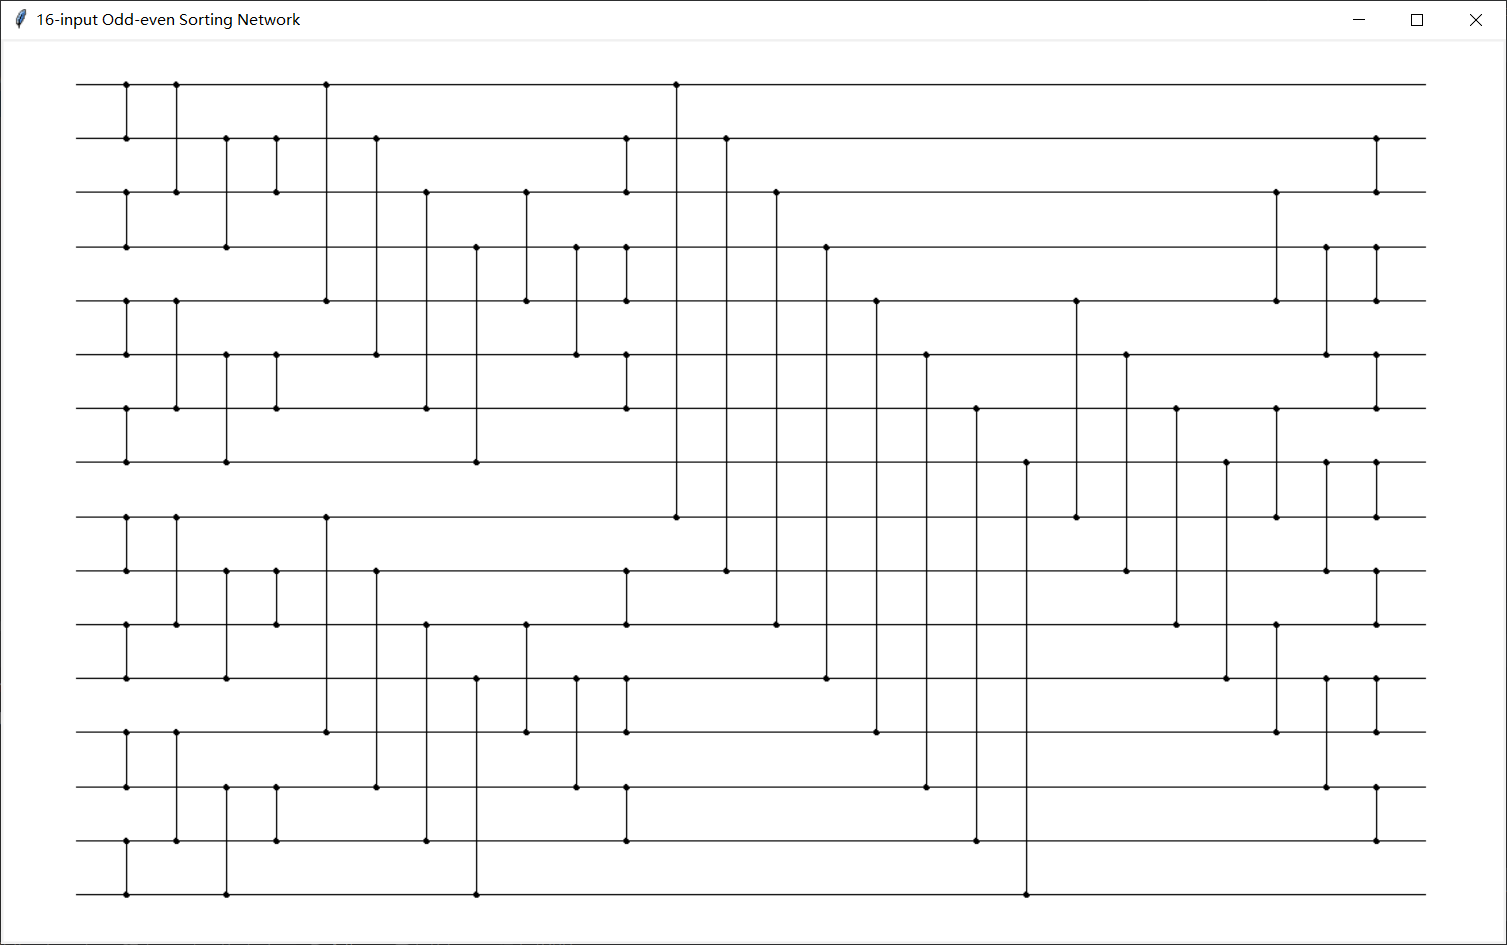
\includegraphics[width=3.1in]{figures/sorting_network_n=8.png}
            \end{minipage}
        }
        \subfigure[$n = 16$]{
            \begin{minipage}[t]{0.45\linewidth}
            \centering
            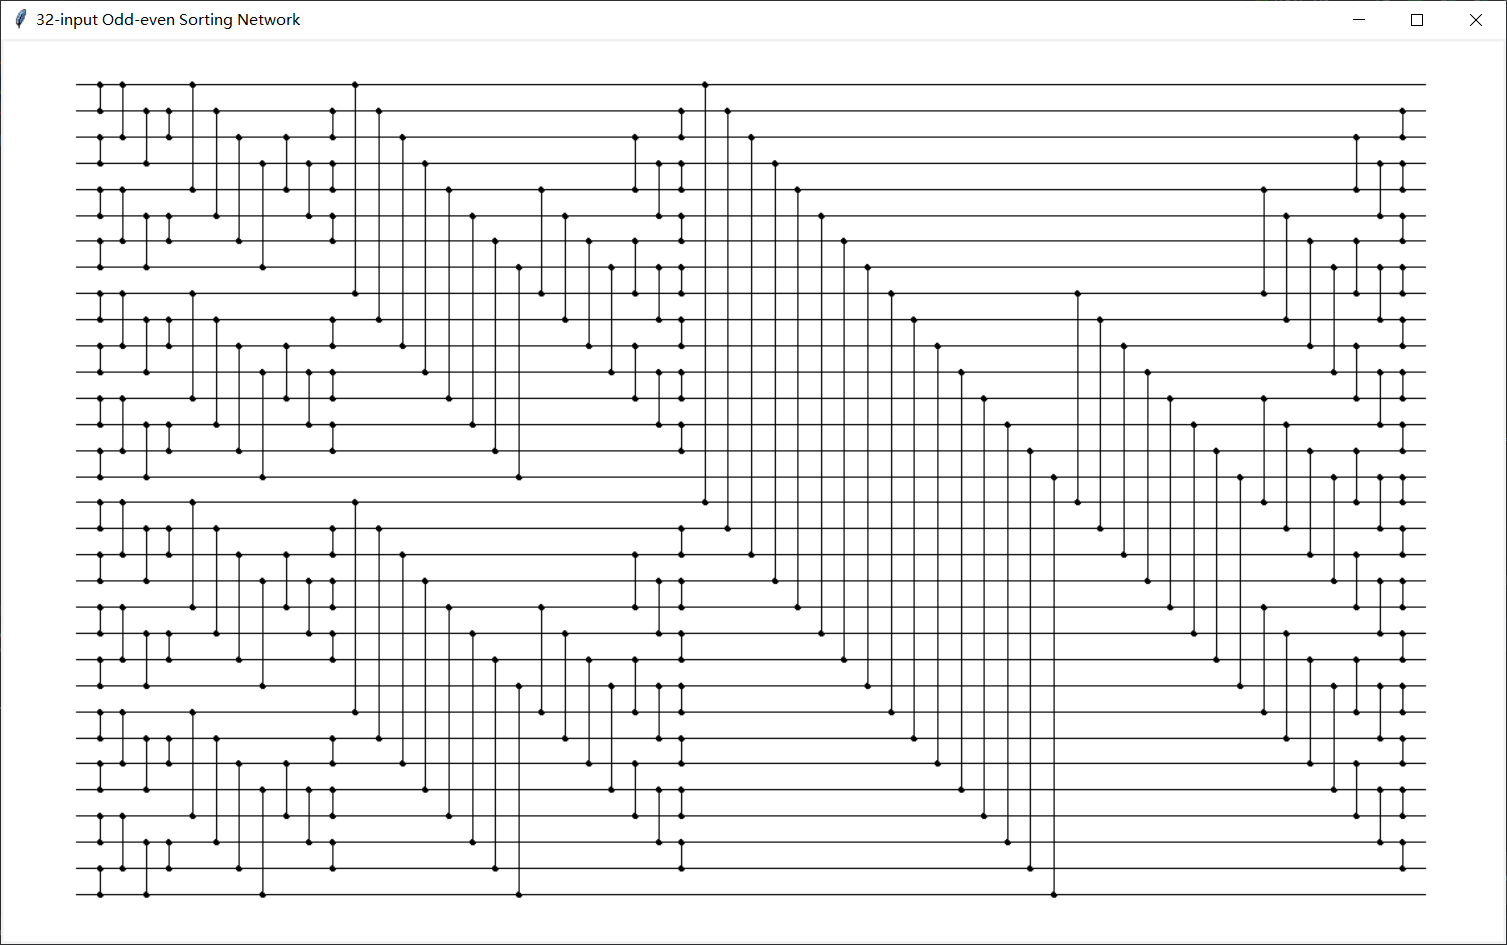
\includegraphics[width=3.1in]{figures/sorting_network_n=16.png}
            \end{minipage}
        }

        \subfigure[$n = 32$]{
            \begin{minipage}[t]{0.45\linewidth}
            \centering
            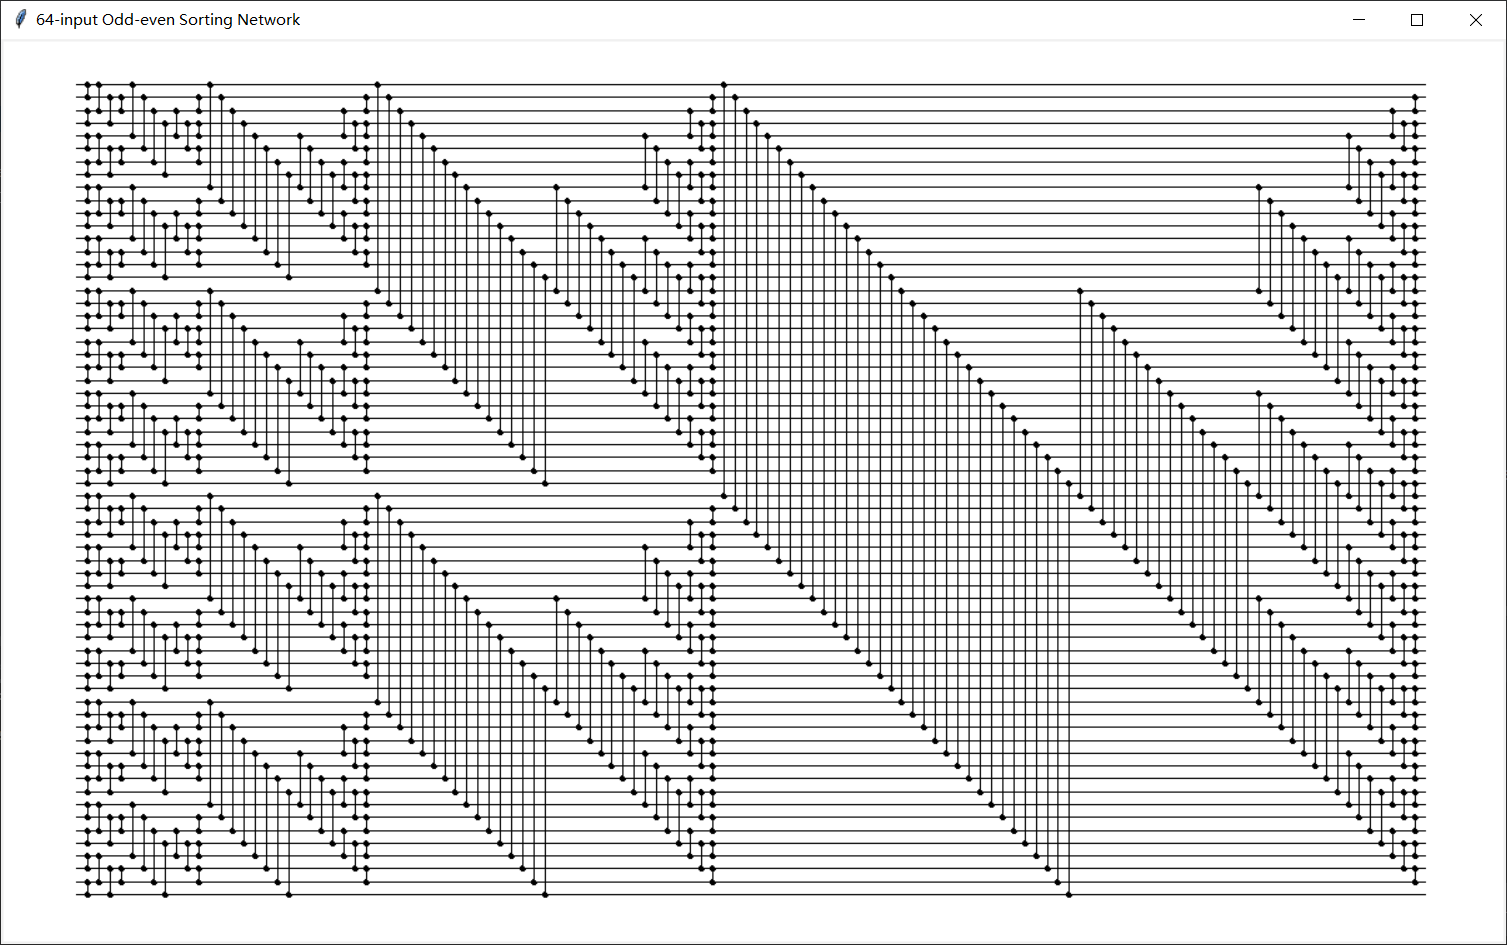
\includegraphics[width=3.1in]{figures/sorting_network_n=32.png}
            \end{minipage}
        }
        \subfigure[$n = 64$]{
            \begin{minipage}[t]{0.45\linewidth}
            \centering
            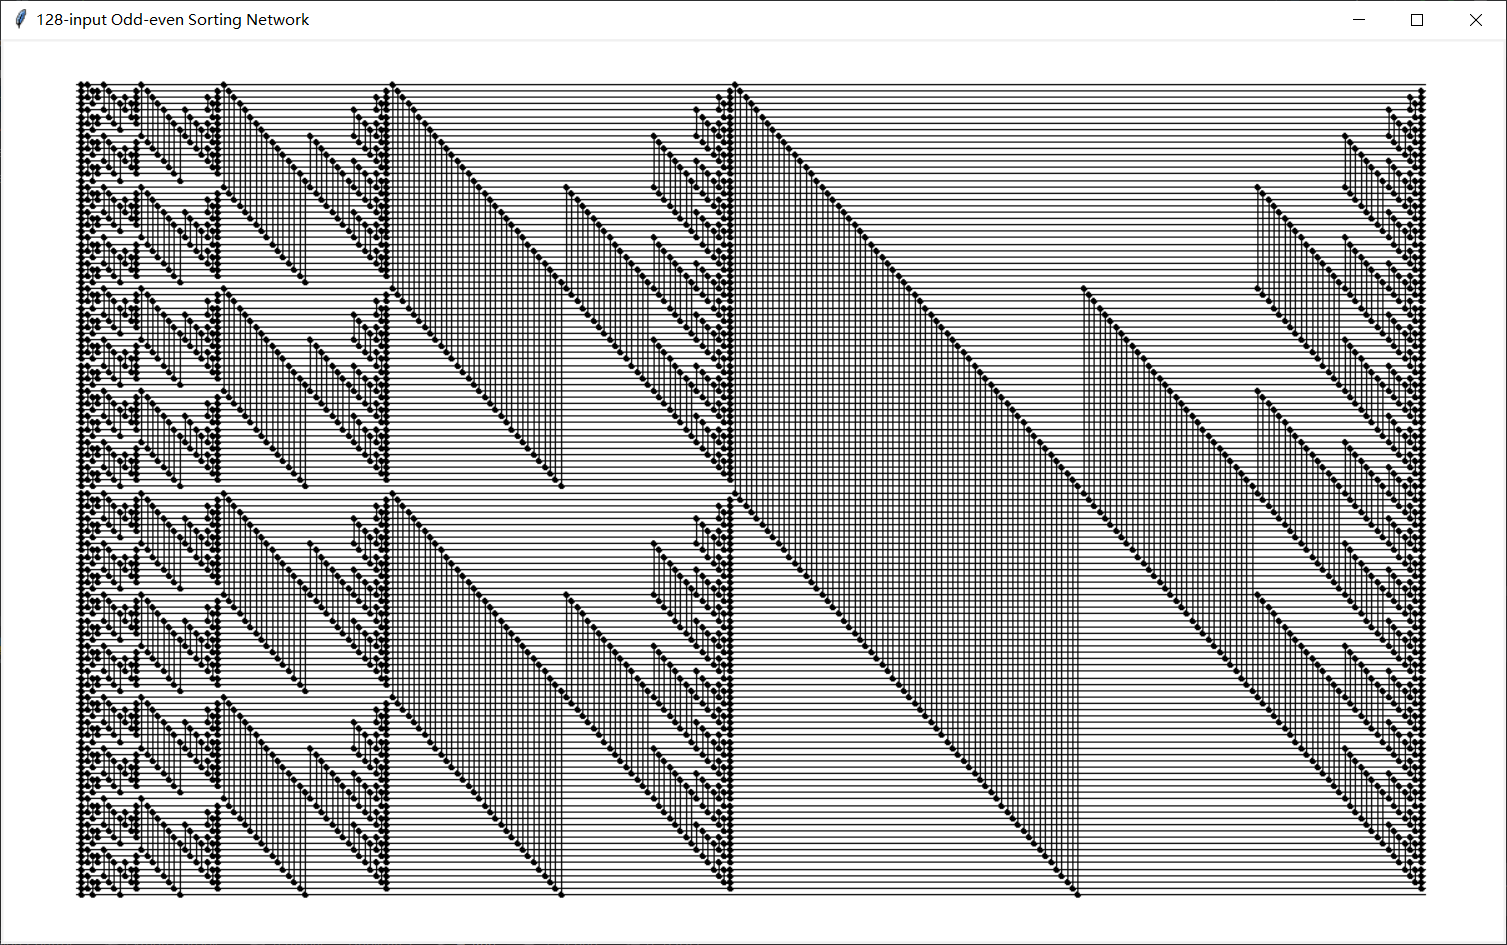
\includegraphics[width=3.1in]{figures/sorting_network_n=64.png}
            \end{minipage}
        }
        \centering
        \caption{$2n$-input odd-even sorting networks}
        \label{fig:1}
    \end{figure}
    \item Let $D_m(n)$ be the depth of $2n$-input odd-even merging network. Then we have the following equation (Equation \eqref{eq3:1}) according to the definition of odd-even merging network.
        \begin{equation}
        D_m(n) = \left\{
        \begin{aligned}
        & 1 & \quad \quad \mathrm{if\ } n = 1 \\
        & D_m\left(\frac{n}{2}\right) + 1 & \quad \quad \mathrm{if\ } n = 2^k \mathrm{\ and\ } k \geq 1
        \end{aligned}
        \right.
        \label{eq3:1}
        \end{equation}
        It is obvious that $D_m(n) = O(\log{n})$.

        Let $D(n)$ be the depth of $2n$-input odd-even sorting network. Then we have the following equation (Equation \eqref{eq3:2}).
        \begin{equation}
        D(n) = \left\{
        \begin{aligned}
        & 1 & \quad \quad \mathrm{if\ } n = 1 \\
        & D\left(\frac{n}{2}\right) + D_m(n) & \quad \quad \mathrm{if\ } n = 2^k \mathrm{\ and\ } k \geq 1
        \end{aligned}
        \right.
        \label{eq3:2}
        \end{equation}
        Suppose $n = 2^k\ (k \ge 1)$, then we can solve the recurrence equation (Equation \eqref{eq3:2}) as follows (Equation \eqref{eq3:3}).
        \begin{equation}
        \begin{aligned}
        D(n) &= D\left(\frac{n}{2}\right) + O(\log{n}) \\
             &= D\left(\frac{n}{4}\right) + O\left(\log{\frac{n}{2}}\right) + O\left(\log{n}\right) \\
             &= ... \\
             &= 1 + \sum_{i=0}^{k-1} O\left(\log{\frac{2^k}{2^i}}\right) \\
             &= O(k^2) \\
             &= O(\log^2{n}) \quad \quad (n = 2^k, k \ge 1)
        \end{aligned}
        \label{eq3:3}
        \end{equation}
        Thus, the depth of the $2n$-input odd-even sorting network is $D(n) = O(\log^2{n})$.
    \item Suppose all the sequences we will discuss later are indexed from $1$.
        \begin{lemma}
            \label{lemma1}
            Suppose there is a sorted 01-sequence of even length, and the even-indexed $1$'s and odd-indexed $1$'s of the sequence are $n_{even}$ and $n_{odd}$ respectively. Then we have $n_{odd} \leq n_{even} \leq n_{odd} + 1$.
        \end{lemma}
        \begin{proof}
            The $1$'s must be placed in \textbf{the last few continuous places} of the sorted $01$-sequence. On one hand, the last place of the sequence is even-indexed, because the sequence has an even length and it is indexed from $1$. Therefore, the even-indexed $1$'s can not be less than the odd-indexed $1$'s, that is, $n_{even} \geq n_{odd}$. On the other hand, $n_{even}$ cannot exceed $n_{odd} + 1$, since the $1$'s in the sequence are continuous. Therefore, we can get $n_{odd} \leq n_{even} \leq n_{odd} + 1$.
        \end{proof}
        \begin{theorem}
            \label{theorem2}
            Let $Q(k)$ be the statement that the $2^k$-input odd-even merging network can merge two sorted $01$-sequences with the same length into one correctly. Then $Q(k)$ is true for every $k \geq 1$.
        \end{theorem}
        \begin{proof} Let us prove the theorem by induction.
            \begin{itemize}
            \item {\color{blue} \textbf{Basis step.}} $Q(1)$ is obviously true, since the $2$-input merging network only contains a comparator and it can merge two sorted $01$-sequences of length $1$ into one correctly.
            \item {\color{blue} \textbf{Induction Hypothesis.}} Assume $Q(i)$ is true for some $i \geq 1$, that is, a $2^i$-input odd-even merging network can merge two $01$-sequences of length $2^{i-1}$ into one correctly.
            \item {\color{blue} \textbf{Proof of Induction Step.}} Now let's prove $Q(i+1)$ is true. A $2^{i+1}$-input odd-even merging network includes two $2^i$-input odd-even merging networks, which can sort the even-indexed part and the odd-index part of the sequence. Suppose the number of even-indexed $1$'s and odd-indexed $1$'s are $n_{even}$ and $n_{odd}$ respectively after sorting the even-indexed sub-sequence and the odd-indexed sub-sequence. According to Lemma \ref{lemma1}, there are only three situations of the two sorted halves (the first half and the second half) in the beginning, which are shown in Fig. \ref{fig:2} (the blue block stands for $1$ in the sequence while the white block stands for $0$ in the sequence).
            \begin{itemize}
            \item \textbf{Situation a:} (Fig. \ref{fig:2a}) In one half, the number of even-indexed $1$'s is greater than the number of odd-indexed $1$'s; in the other half, the number of even-indexed $1$'s equals to the number of odd-indexed $1$'s. According to the previous lemma, after sorting the odd-indexed sub-sequence and even-indexed sub-sequence respectively, we have $n_{even} = n_{odd} + 1$. After combining two sub-sequence together, the $1$'s are all in the last continuous places of the sequence (i.e., the sequence looks like $00...011...1$). Thus the sequence is sorted.
            \item \textbf{Situation b:} (Fig. \ref{fig:2b}) The number of even-indexed $1$'s equals to the number of the odd-indexed $1$'s in both two parts. According to the previous lemma, after sorting the odd-indexed sub-sequence and even-indexed sub-sequence respectively, we have $n_{even} = n_{odd}$. After combining two sub-sequence together, the $1$'s are all in the last continuous places of the sequence (i.e., the sequence looks like $00...011...1$). Thus, the sequence is sorted.
            \item \textbf{Situation c:} (Fig. \ref{fig:2c}) The number of even-indexed $1$'s is greater than the number of the odd-indexed $1$'s in both two parts. According to the previous lemma, after sorting the odd-indexed sub-sequence and even-indexed sub-sequence respectively, we have $n_{even} = n_{odd} + 2$. After combining two sub-sequence together, most of the $1$'s are all in the last continuous places of the sequence and only an $1$ is located in a places before the last continuous $1$'s (i.e., the sequence looks like $00...01011...1$). Then we perform the last step of the merging network: use comparators between the odd-indexed and the even-indexed. The sequence will be sorted after the process, since the special $1$ is even-indexed and it will be swapped with the $0$ between $1$'s.
            \end{itemize}
            \begin{figure}[h]
                \centering
                \subfigure[Situation a] {
                    \begin{minipage}[t]{0.3\linewidth}
                        \centering
                        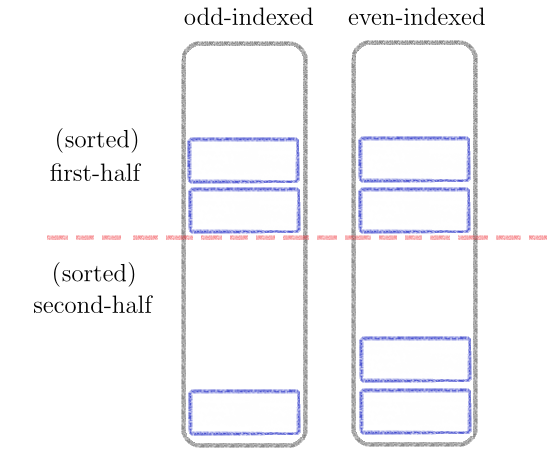
\includegraphics[width=2.4in]{figures/merger-proof-1.png}
                    \end{minipage}
                    \label{fig:2a}
                }
                \subfigure[Situation b] {
                    \begin{minipage}[t]{0.3\linewidth}
                        \centering
                        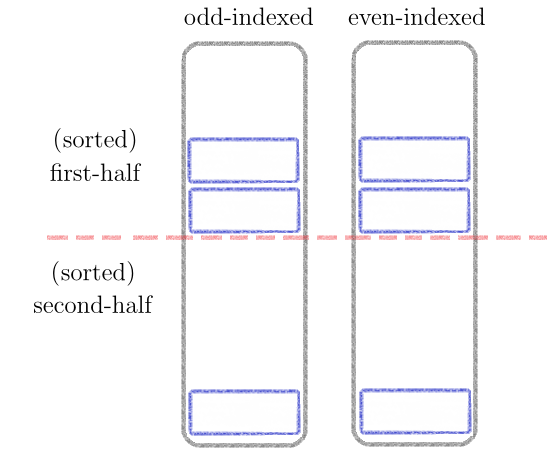
\includegraphics[width=2.4in]{figures/merger-proof-2.png}
                    \end{minipage}
                    \label{fig:2b}
                }
                \subfigure[Situation c] {
                    \begin{minipage}[t]{0.3\linewidth}
                        \centering
                        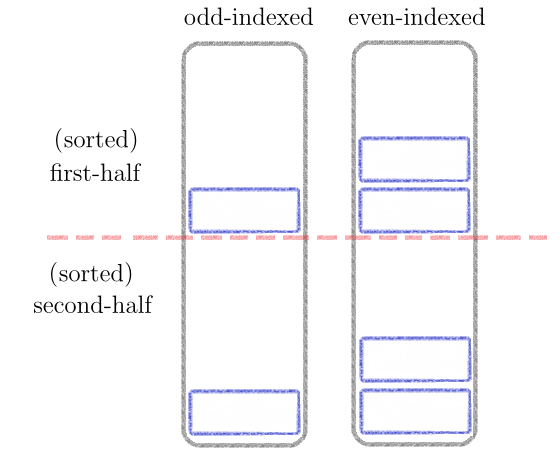
\includegraphics[width=2.4in]{figures/merger-proof-3.png}
                    \end{minipage}
                    \label{fig:2c}
                }
                \caption{Sequence before merging}\label{fig:2}
            \end{figure}
                In summary, two sorted $01$-sequences with the same length will be merged into a sorted sequence after putting it into the $2^{i+1}$-input odd-even merging network. Thus $Q(i+1)$ is true.
            \end{itemize}
        \end{proof}

        Suppose $n = 2^k\ (k \geq 0)$. According to Theorem \ref{theorem2}, we know that $Q(k+1)$ is true, that is, two sorted $01$-sequences with the same length will be merged into a sorted sequence after putting it into the $2^{k+1}$-input odd-even merging network. Hence, we prove that the $2n$-input odd-even merging network is indeed a merging network, since $2n = 2^{k+1}$.

        According to \textbf{the zero-one principle}, we know that any $2n$-input odd-even merging network is indeed a merging network.
    \end{enumerate}
    \end{solution}

\end{enumerate}

\vspace{20pt}

\textbf{Remark:} You need to include your .pdf, .tex and .py files (or other possible sources) in your uploaded .rar or .zip file.

%========================================================================
\end{document}
